% Исходный LaTeX-код (c) Пётр Калинин
% Код распространяется по лицензии GNU GPL (!)

\header{Простые задачи, решаемые поиском в глубину}
В этом разделе почти везде будем рассматривать только неориентированные графы.
\lheader{Компоненты связности графа}
Довольно очевидно доказывается, что поиск в глубину, запущенный из некоторой вершины графа, обойдёт все вершины
из той компоненты связности, в которой находится наша вершина.

Докажем это. Действительно, пусть есть вершина, лежащая в той же 
компоненте\footnote{Кстати, грамматический вопрос: какого рода слово "<компонента">? Вроде очевидно 
женского, но не является ли это ошибкой, ведь нормальное слово"=то "--- компонент (прибора, например)? На самом деле в 
соответствующих словарях чётко зафиксировано выражение \textit{компонента связности}, 
\textit{компонента вектора} и т.п., так что в математике это вроде не ошибка.}
связности, но до которой мы не дошли.
Раз она лежит в той же компоненте связности, то есть путь из начальной вершины в неё. В начальной вершине пути мы точно побывали (мы ведь оттуда запустились), в конечной вершине нет (по предположению). Тогда очевидно, что вдоль пути найдутся
две \textit{соседние} вершины $u$ и $v$ такие, что в $u$ мы побывали, а в $v$ нет. Раз они соседние в нашем пути, то они
соединены ребром. Тогда спрашивается: что мы делали, когда просматривали соседей вершины $u$? Почему не пошли в $v$? 
Противоречие, следовательно, мы действительно обойдём всю соответствующую компоненту связности.

\note{Как видите, доказательство от противного. Мне кажется, что это довольно хорошо подчёркивает саму суть 
поиска в глубину: сразу далеко не очевидно, что оно работает. Попытки в лоб доказать, что оно работает, не пройдут.
Но тем не менее оно действительно работает.}

Естественно, мы считаем, что перед запуском массив $was$ по крайней мере в пределах этой компоненты связности был 
заполнен нулями, иначе, конечно, ничего не получится.

\task|Понимаете, почему может ничего не получиться, если массив $was$ изначально неправильно заполнен?
Заодно что вы можете сказать по поводу проверки \emph{ориентированного} графа на связность?||||Ясно, что, если в текущей компоненте связности некоторые элементы массива $was$ изначально были 
ненулевыми, то в эти вершины мы не войдём. Скорее всего, это немного не то, что мы хотели (хотя, конечно,
все зависит от задачи. Могут быть задачи, хотя я таких с ходу не припомню, в которых нам именно это и надо).|\label{fillwas}

Таким образом, чтобы проверить, что граф (неориентированный!) связен, поступаем очень просто: запускаем поиск в 
глубину из любой вершины и после этого проверяем, что мы побывали во всех вершинах:

\begin{codesampleo}\begin{verbatim}
fillchar(was,sizeof(was),0);
find(1);
for i:=1 to n do
    if was[i]=0 then
       writeln('Non-connected!');
\end{verbatim}
\end{codesampleo}

Пусть теперь нам надо найти все компоненты нашего (возможно, не связанного) графа. Т.е. нам надо посчитать их, а в
специальный массив для каждой вершины записать номер соответствующей компоненты. Я думаю, это тоже вполне понятно.
Запускаемся из первой вершины, потом ищем ещё непосещённую вершину и запускаемся из неё и т.д. Правда, некоторую сложность
может составить реализация этого дела, но, если немного подумать, то можно написать так:
\begin{codesample}\begin{verbatim}
procedure find(i:integer);
var j:integer;
begin
if was[i]<>0 then
   exit;
was[i]:=nc;
for j:=1 to n do
    if gr[i,j]=1 then
       find(j);
end;

begin
nc:=0;
fillchar(was,sizeof(was),0);
for i:=1 to n do
    if was[i]=0 then begin
       inc(nc);
       find(i);
    end;
end.
\end{verbatim}
\end{codesample}

Здесь $nc$ "--- глобальная переменная, хранящая количество уже найденных компонент связности. Номер компоненты связности,
как я и обещал выше, мы записываем прямо в массив $was$: компоненты мы нумеруем, начиная с 1, поэтому проблем не возникает.
$was[i]=0$ обозначает, что вершина $i$ ещё не была посещена, иначе вершина была посещена, а $was[i]$ "--- номер
её компоненты связности. Поэтому в процедуре мы делаем именно $was[i]:=nc$, а не 1, как раньше.

Ещё обратите внимание, что тут \textit{обязательно} нужна проверка \texttt{if was[i]=0} в главной программе, даже
несмотря на то, что соответствующая проверка написана \textit{в начале} процедуры. Действительно, проверка в главной
программе нужна, чтобы не увеличить число компонент лишний раз.

И наконец заметьте, что, конечно, массив $was$ мы инициализируем один раз за программу.

\lheader{Проверка графа на двудольность}
$N$"=дольным называется неориентированный граф, вершины которого можно раскрасить в $N$ цветов так, что концы любого 
ребра будут разноцветными, т.е. не будет рёбер, ведущих из одного цвета в тот же самый цвет. В 
таком случае группы вершин одного цвета называются \textit{долями} графа. В частности, двудольный 
граф "--- граф, вершины которого можно разбить на две группы"=доли так, что каждое ребро будет 
вести из одной доли в другую.

Нередко двудольные графы являются двудольными по 
своей природе, т.е. нередко сама природа вершин разных долей разная: классический пример "--- 
первая доля "--- люди (работники), вторая "--- работы, которые они могут выполнять, ребро между 
человеком и работой есть, если он умеет её выполнять. Очевидно, что тут ребра в пределах одной доли 
совершенно бессмысленно. В таких случаях обычно сразу во входном файле задаётся граф так, что он не 
может оказаться недвудольным, и вообще вопрос о проверке графа на двудольность бессмысленен. Но 
бывает так, что дан просто граф, а надо проверить, является ли он двудольным. Именно такую задачу мы 
и будем рассматривать здесь. Одновременно с проверкой на двудольность мы сразу будем находить его 
доли. 

\task|Может ли эта задача иметь несколько решений? Т.е. может ли быть так, что 
разбиение вершин графа на доли неоднозначно? Попробуйте сформулировать как можно более простой 
критерий, который отвечает на этот вопрос. Только, прежде чем читать дальше, ответьте на это 
задание.||||Да, конечно, количество решений равно $2^k$, где $k$ "--- количество компонент связности графа.
В пределах одной компоненты есть два способа раскраски, отличающиеся инвертацией всех вершин. 

Вообще, есть элементарная неоднозначность: можно инвертировать все вершины сразу и получить новое решение "---
значит, решение \textit{всегда} неоднозначно. Но даже если решения, отличающиеся инвертацией \textit{всех} вершин, 
считать одинаковыми, то все равно в несвязных графах решение неоднозначно.|\label{ambigousbi}

Итак, нам дан граф. Давайте попробуем его покрасить. Возьмём первую вершину и покрасим её в какой 
попало цвет (т.е. отнесём её к какой попало доле). Тогда сразу понятно, как надо красить соседние с 
ней вершины. Покрасим их как надо. После этого понятно, как надо красить соседние с ними вершины и 
т.д. (Довольно сильно напоминает волновой алгоритм.) Так будет продолжаться до тех пор, пока не 
случится одно из двух:

1. Возникнет противоречие, т.е. мы должны будем покрасить одну и ту же вершину в разные цвета 
одновременно или должны будем \textit{перекрашивать} уже покрашенную вершину. Что это обозначает? 
Единственный произвол, который мы делали, состоял в выборе цвета самой первой вершины. Очевидно, 
что, если мы попробуем другой вариант цвета первой вершины, то противоречие сохранится, просто 
цвета всех покрашенных вершин инвертируются. Тогда очевидно, что граф не двудольный.

2. Нам будет нечего делать, т.е. мы покрасили несколько вершин, противоречий нет, но ни у одной из 
уже покрашенных вершин нет непокрашенных соседей. Что это значит? Одно из двух: либо мы покрасили 
весь граф "--- круто, задача решена, ответ положительный (\taskn{Контрольный вопрос}|Ответ на 
какой вопрос? :) ||||Конечно, на вопрос "<является ли данный граф двудольным">.|\label{whichtask}).  
Либо есть ещё непокрашенные вершины. Но ясно, что тогда они находятся в 
\textit{другой} компоненте связности и потому их можно красить \textit{независимо} от уже 
покрашенных. Возьмём любую из ещё непокрашенных вершин и покрасим её как попало и т.д., продолжая 
как описано выше. Опять либо возникнет противоречие, тогда граф точно не двудольный, т.к. на это 
противоречие влиял только самый последний произвол, а его инвертировать опять бессмысленно (а 
предыдущие выборы, которые мы делали, не имеют теперь значения), либо опять будет нечего красить 
"--- аналогично либо все покрасили, либо переходим к третьей компоненте и т.д.

Таким образом в конце концов мы или покрасим весь граф, или придём к выводу, что граф не 
двудольный. Прежде чем обсуждать реализацию, обсудим ещё небольшой теоретический вопрос.

Можно ли придумать какой"=нибудь критерий двудольности графа? Давайте подумаем, когда 
"<затыкается"> наш алгоритм. Когда обнаруживает противоречие, т.е. одну и ту же вершину пытается 
сразу покрасить и в белый, и в чёрный цвет. Говоря по другому, когда у одной ещё непокрашенной 
вершины находятся два \textit{разноцветных} соседа. Что это обозначает? До сих пор все было 
нормально, т.е. на каждом ребре цвет чередовался, поэтому цвета обозначают фактически "<слои"> 
графа: до вершин одного цвета от начальной мы добираемся за чётное число шагов (рёбер), до вершин второго 
цвета "--- за нечётное. Если же появилось противоречие, значит, нашлась вершина, до которой мы 
можем добраться и за чётное, и за нечётное количество шагов. Это обозначает, что появился 
\textit{цикл нечётной длины}: от начальной вершины до неё самой можно добраться за \textit{нечётное} 
количество шагов. Очевидно, что в двудольном графе не может быть циклов нечётной длины: в любом 
цикле вершины разных долей чередуются, и потому, чтобы вернутся в начальную вершину, надо сделать 
\textit{чётное} количество шагов. Поэтому ясно, что, раз наш алгоритм нашёл"=таки такой цикл, то 
граф точно недвудольный. А теперь заметим самое главное: если циклов нечётной длины в графе точно 
нет, то наш алгоритм в принципе не сможет "<заткнуться">, т.е. он корректно раскрасит граф, т.е. 
граф двудольный. Таким образом, мы доказали это утверждение в обе стороны: граф двудольный тогда и 
только тогда, когда в нем нет циклов нечётной длины.

Все то же самое, но по"=другому изложенное (это изложение, может быть, сложнее с ходу понять, и тем 
более не понятно, как до него дойти, но зато оно очень хорошо помогает разложить все по полочкам, 
чтобы быть уверенными, что мы нигде ничего не сглючили):

\textbf{Теорема} (о двудольности графа)\textbf{:} \textit{граф двудольный тогда и только тогда, когда в нем 
нет циклов нечётной длины.}

\textbf{Доказательство:}

$\underline{\Rightarrow}$ Пусть граф двудольный. Тогда в нем вдоль каждого цикла цвета вершин 
чередуются, поэтому цикл обязательно имеет чётную длину.

$\underline{\Leftarrow}$ Пусть в графе нет циклов нечётной длины. Запустим вышеприведённый 
алгоритм. Он может остановиться, найдя противоречие, только если найдёт цикл нечётной длины, что 
невозможно. Следовательно, он корректно раскрасит граф, значит, граф двудольный. \textsc{чтд.}

Обратите внимание, что доказательство в одну сторону сильно отличается от доказательства в 
обратную. Ещё обратите внимание, что отсюда очевидно следует, что дерево (и вообще лес) "--- 
двудольный граф.

\vspace{0.2cm}


Как теперь реализовать этот алгоритм? Напрашивающаяся идея "--- поиск в ширину, он же волновой 
алгоритм. Вполне можно. 

\task|Реализуйте этот алгоритм с помощью поиска в ширину.||||Ну что"=нибудь в следующем стиле (конечно, поиск в ширину я реализую очередью)
\begin{codesample}\begin{verbatim}
var q:array[1..n] of integer;
    was:array[1..n] of integer;
    l,r:integer;
    cur:integer;
    j:integer;
...
fillchar(was,sizeof(was),0);
l:=1;r:=1;
q[1]:=1;
was[1]:=1;
while l<=r do begin
      cur:=q[l];
      inc(l);
      for j:=1 to n do
          if (gr[cur,j]<>0)and(was[j]=0) then begin
             was[j]:=3-was[cur];
             inc(r);
             q[r]:=j;
          end;
end;
\end{verbatim}
\end{codesample}
Массив $q$ "--- очередь, массив $was$ "--- номера доли. Это работает для связного графа, в противном случае ещё
нужен внешний цикл с проверкой $was$. Надеюсь, тут ошибок немного.|\label{BFS:bipartie}

Но если немного подумать, то подойдёт \textit{любой} обход  графа, который переходит из одной 
вершины в другую только по рёбрам и обходит весь граф. Например, вполне подойдёт поиск в глубину; 
поскольку поиск в глубину реализовать обычно проще, чем в ширину, то обычно проверяют граф на 
двудольность с помощью поиска в глубину.

Итак, каждый раз, когда находим новую вершину, будем её красить в нужный цвет.
\begin{codesample}
\begin{verbatim}
procedure find(i:integer);
var j:integer;
begin
for j:=1 to n do
    if gr[i,j]=1 then begin
       if was[j]=was[i] then begin
          ok:=false;
          exit;
       end;
       if was[j]<>0 then
          continue;
       was[j]:=3-was[i];
       find(j);
       if not ok then
          exit;
    end;
end;

...
fillchar(was,sizeof(was),0);
ok:=true;
for i:=1 to n do
    if was[i]=0 then begin
       was[i]:=1;
       find(i);
       if not ok then
          break;
    end;
\end{verbatim}
\end{codesample}

Итак, что тут. Массив $was$ опять используем для хранения дополнительной информации: в данном 
случае цвета вершины (1 или 2). Может быть, логичнее его было бы назвать как"=нибудь по"=другому.
В процедуре $find$, когда находим очередного соседа текущей вершины, смотрим: если он того же 
цвета, что и мы, то облом, иначе если он уже покрашен, то туда не сунемся, иначе красим ($3-was[i]$ 
даёт как раз нужный цвет) и запускаем поиск из этой вершины. Обратите внимание, что красим вершину 
(т.е. заполняем $was[j]$) мы \textit{до} входа в процедуру $find(j)$, поэтому в начале процедуры 
ничего вообще не делаем. В главной программе теперь найдя ещё непокрашенную вершину, красим её 
(обязательно! т.к. не красим её в самой процедуре) и запускаемся. Обратите внимание, как сделана 
работа с переменной $ok$, которая хранит, не наши ли мы ещё противоречия.

Какой"=то ужас тут получается. Поэтому имхо логичнее перенести всю работу в начало процедуры, а 
"--- внимание! "--- в процедуру будем передавать \textit{дополнительный} параметр "--- цвет, в 
который надо покрасить эту вершину.
\begin{codesample}
\begin{verbatim}
procedure find(i,c:integer);
var j:integer;
begin
if was[i]<>0 then begin
   if was[i]<>c then
      ok:=false;
   exit;
end;
was[i]:=c;
for j:=1 to n do
    if gr[i,j]=1 then begin
       find(j,3-c);
       if not ok then
          exit;
    end;
end;

...
fillchar(was,sizeof(was),0);
ok:=true;
for i:=1 to n do
    if was[i]=0 then begin
       find(i,1);
       if not ok then
          break;
    end;
\end{verbatim}
\end{codesample}

Теперь работа процедуры $find$ имхо более очевидна: она пытается покрасить вершину $i$ в цвет $c$. 
Во"=первых, если вершина уже покрашена, то надо только посмотреть, в тот ли цвет (обратите 
внимание, что в прошлом варианте была проверка $was[i]=was[j]$, а теперь $was[i]<>c$), и выйти. 
Иначе красим и смотрим соседей.

Ещё замечу, что, если в случае, когда граф недвудольный, нужно сделать что"=то простое и завершить 
работу программы (например, вывести `\texttt{No solution}' и выйти), то можно с $ok$ не возиться, а 
просто сделать что надо:
\begin{codesample}
\begin{verbatim}
procedure outno;
begin
...
halt;
end;


procedure find(i,c:integer);
var j:integer;
begin
if was[i]<>0 then begin
   if was[i]<>c then outno;
   exit;
end;
was[i]:=c;
for j:=1 to n do
    if gr[i,j]=1 then begin
       find(j,3-c);
    end;
end;
\end{verbatim}
\end{codesample}

Ещё замечу, что можно переменную $ok$ убрать, а процедуру $find$ сделать функцией, возвращающей boolean. Можете 
попробовать это реализовать. Наконец, если гарантируется, что граф двудольный, надо только его доли 
найти, то $ok$ вообще не нужна.

\task|А почему также нельзя проверять граф на трехдольность?||||Ну понятно, почему :) Для двудольности, 
покрасив одну вершину, мы тут же знаем, как красить
соседние с ней, т.к. есть всего два варианта, а один из них уже занят. В трехдольности так не получится.|\label{tripartie}

\lheader{Проверка, является ли граф деревом}
Как вы знаете, деревом называется связный граф без циклов (все ещё рассматриваем только 
неориентированные графы), лесом называется произвольный, т.е. не обязательно связный, граф без 
циклов. Как проверить, является ли граф деревом или лесом? В принципе, понятно: проверить, что 
циклы в графе отсутствуют, можно просто запустив поиск в глубину и посмотрев, не придём ли мы 
когда"=нибудь в ту вершину, где мы уже побывали.

Конкретно: если нам надо проверить, является ли граф деревом, то запустимся из первой вершины. Если 
хоть раз вернёмся в вершину, где мы уже побывали, то граф точно не дерево. Иначе в конце проверим, 
верно ли, что мы побывали во всех вершинах. Если да, то граф связен, а отсутствие циклов мы уже 
проверили "--- ок. Иначе не дерево.

Если нам надо проверить, является ли граф лесом, то все аналогично, только аналогично поиску всех 
компонент связности закончив поиск в глубину из первой вершины, запускаемся из первой ещё не 
посещённой и т.д. "--- такой же цикл, как и при поиске компонент связности.

\task|Напишите эти две программы. Тщательно потестируйте их. Переберите все возможные 
подлые случаи. Представьте, что вы "--- жюри на некоторой олимпиаде и даёте участникам такую 
задачу. Вы знаете, как её решать, поэтому можете продумать, какие тут подлости возможны "--- на них 
и делайте тесты. Например, очевидно, надо оттестировать связные и несвязные графы; деревья, леса, 
несвязные графы, у которые первая компонента является/не является деревом; линейные структуры (т.е. 
первая вершина связана со второй, вторая "--- с третьей и т.д.) и разветвлённые деревья; длинные 
циклы, пустые графы и т.д. 

При написании программы почти наверняка вы столкнётесь с (одним) большим подводным камнем. Осознайте его, 
поймите, почему ваша программа не работает, и исправьте программу так, чтобы она работала.

Текст программы тут я приводить не буду, приведу только в ответах. У этой задачи есть подсказка;
порешав задачу, посмотрите подсказку до ответа.
||Подводный камень, с которым вы столкнётесь "--- это то, что из каждой вершины
вы будете пытаться пойти в вершину"=родителя текущей вершины и программа будет считать, что она нашла цикл, 
хотя на самом деле это "--- не цикл. Самый простой способ, который я знаю, чтобы избежать этой проблемы
"--- это передавать в процедуру find дополнительный параметр "--- вершину"=родителя текущей вершины "--- и 
перед рекурсивным вызовом проверять, не является ли та вершина, куда мы пытаемся пойти, родителем текущей.
||Собственно, в подсказке я уже сказал, как надо все делать. Осталось привести пример программы.
\begin{codesampleo}\begin{verbatim}
procedure find(i,p:integer);
begin
if was[i]<>0 then begin
   не дерево!
   exit;
end;
was[i]:=1;
for i:=1 to n do
    if (gr[i,j]=1)and(j<>p) then
       find(j,i);
end;
\end{verbatim}
\end{codesampleo}
Дополнительный параметр $p$ здесь "--- номер вершины"=предка. Вызываем эту процедуру из главной программы, 
конечно, передавая в качестве 
вершины"=предка номер несуществующей вершины, например, ноль, если нумеруем вершины с единицы.

Да, ещё не забудьте, что для проверки, является ли граф деревом, надо запустить $find(1)$ и проверить, что вы побывали
во всех вершинах, а для проверки, является ли граф лесом, надо пробежаться по всем вершинам и запускать $find$
оттуда, где ещё не бывали.|\label{checkiftree}

\lheader{Нахождение эйлерова пути и цикла}
Я думаю, вы знаете, что такое эйлеров цикл "--- это цикл, который проходит по каждому ребру ровно 
один раз. Аналогично, эйлеров путь "--- это путь, который по каждому ребру проходит ровно один раз 
(но, в отличии от цикла, может начинаться и заканчиваться в разных вершинах). Я также думаю, что вы 
знаете критерий наличия эйлерова цикла и эйлерова пути в графе. Действительно, если в графе есть 
эйлеров цикл, то в при движении по нему в каждую вершину мы входим ровно столько же раз, сколько 
выходим. За время прохода по всему циклы мы прошли по все рёбрам, инцидентным данной вершине, 
следовательно, степень каждой вершины \textit{должна быть} чётна (мы пока все ещё рассматриваем 
неориентированные графы). Совершенно аналогично, если в графе есть эйлеров путь, то степени только 
двух вершим могут быть нечётны "--- это будут начало и конец нашего пути: из начала мы вышли на 
один раз больше, чем вошли в него, с концом пути все наоборот. Ещё, очевидно, надо поставить некоторое 
условие на связность графа. Мы будем дальше считать граф связным, но это не есть 
\textit{необходимое} условие.

\task|Попробуйте сформулировать это условие абсолютно точно, т.е. указать, какое условие на 
связность графа надо добавить к условию на степени вершин, чтобы получить критерий существования 
эйлерова цикла/пути в графе, такой, что, если он выполняется, то путь/цикл точно есть, иначе точно 
нет.||Могут существовать несвязные графы, в которых эйлеров цикл все"=таки существует.||Окончательный критерий "--- если 
в графе степени всех вершин чётны плюс все компоненты связности,
кроме, может быть, одной, состоят из одной вершины (т.е. это связный граф и ещё несколько изолированных вершин).|\label{Eulercriteria}

Обратите внимание, что вышеприведённые рассуждения не доказывают \textit{существования} цикла/пути, 
если эти условия выполняются. Существование цикла мы будем доказывать построением алгоритма, 
который будет решать эту задачу. Наш алгоритм будет находить цикл/путь в любом связном графе, 
удовлетворяющим условию на степени вершин (что делать для несвязного графа "--- это ваше задание).

Итак, пусть граф связен и степени всех его вершин чётны. Построим эйлеров цикл. Пожалуй, тут проще 
будет привести сам алгоритм, а потом объяснить, почему он работает. Итак, запустим поиск в глубину, 
но \textit{не} будем контролировать возвращение в уже посещённые вершины: будем допускать сколько 
угодно раз приходить в одну и ту же вершину (очевидно, что в общем случае эйлеров цикл будет через 
каждую вершину проходить по нескольку раз, поэтому ясно, что без этого изменения поиск в глубину не 
поможет). Зато будем стирать ребра из графа, как только мы по ним прошли. Ясно, что тогда алгоритм 
до бесконечности работать не будет. Когда будем \textit{выходить} из вершины, будем выводить её 
номер в выходной файл:
\begin{codesampleo}\begin{verbatim}
procedure find(i:integer);
var j:integer;
begin
for j:=1 to n do
    if gr[i,j]=1 then begin
       gr[i,j]:=0;
       gr[j,i]:=0;
       find(j);
    end;
write(i,' ');
end;
\end{verbatim}
\end{codesampleo}
Обратите внимание, что стираем ребра мы \textit{двумя} присваиваниями, ведь каждому ребру в матрице 
смежности соответствуют две единички.

\begin{wrapfigure}{r}{3cm}
\vspace{-0.3cm}
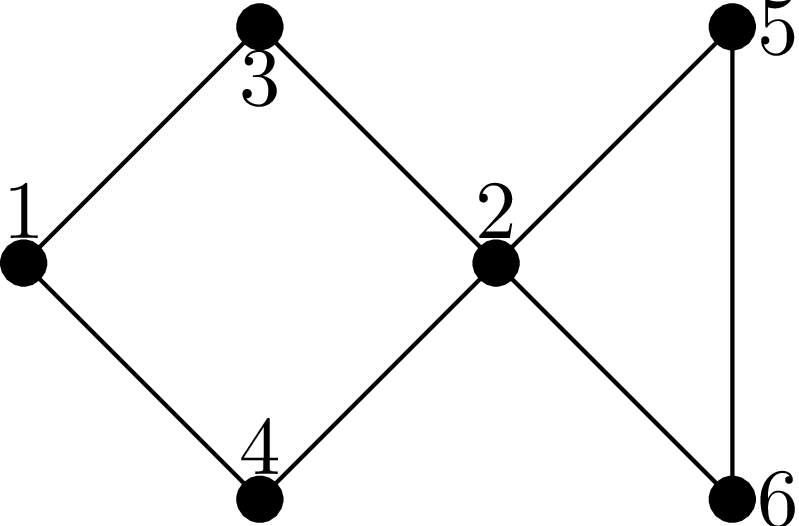
\includegraphics[width=3cm]{texts/04_2_simple/graph.1}
\end{wrapfigure}
Утверждается, что после работы этого алгоритма (точнее, после выполнения команды $find(1)$)
на экран будет выведена последовательность вершин, 
которая образует эйлеров цикл. Чтобы понять это лучше, пожалуй, стоит разобрать простой пример.
Рассмотрим граф, показанный справа "--- в нем, очевидно, есть эйлеров цикл. Как будет работать наш 
алгоритм?

\vspace{0.3cm}

{\newcommand{\ind}{\hspace*{1cm}}\footnotesize\noindent
find(1)\\
нашли соседа "--- вершину 3, стираем ребро 1--3\\
\ind find(3)\\
\ind нашли соседа "--- вершину 2, стираем ребро 3--2\\
\ind \ind find(2)\\
\ind \ind нашли соседа "--- вершину 4, стираем ребро 2--4\\
\ind \ind \ind find(4)\\
\ind \ind \ind нашли соседа "--- вершину 1, стираем ребро 4--1\\
\ind \ind \ind \ind find(1)\\
\ind \ind \ind \ind \textit{(все ребра из вершины 1 уже стёрты, поэтому 
                                      никаких соседей не находим)}\\
\ind \ind \ind \ind \textbf{writeln(1);}\\
\ind \ind \ind \ind завершаем процедуру find(1)\\
\ind \ind \ind \textit{(больше никуда из вершины 4 не идём, т.к. все ребра уже стёрты)}\\
\ind \ind \ind \textbf{writeln(4);}\\
\ind \ind \ind завершаем процедуру find(4)\\
\ind \ind \textit{(продолжаем поиск из вершины 2)}\\
\ind \ind нашли соседа "--- вершину 5, стираем ребро 2--5\\
\ind \ind \ind find(5)\\
\ind \ind \ind нашли соседа "--- вершину 6, стираем ребро 5--6\\
\ind \ind \ind \ind find(6)\\
\ind \ind \ind \ind нашли соседа "--- вершину 2, стираем ребро 6--2\\
\ind \ind \ind \ind \ind find(2)\\
\ind \ind \ind \ind \ind \textit{(больше никуда из вершины 2 не идём, т.к. все ребра уже стёрты)}\\
\ind \ind \ind \ind \ind \textbf{writeln(2);*}\\
\ind \ind \ind \ind \ind завершаем процедуру find(2)\\
\ind \ind \ind \ind \textit{(продолжаем поиск из вершины 6, но ничего больше не находим)}\\
\ind \ind \ind \ind \textbf{writeln(6);}\\
\ind \ind \ind \ind завершаем процедуру find(6)\\
\ind \ind \ind \textit{(больше никуда из вершины 5 не идём, т.к. все ребра уже стёрты)}\\
\ind \ind \ind \textbf{writeln(5);}\\
\ind \ind \ind завершаем процедуру find(5)\\
\ind \ind \textit{(продолжаем поиск из вершины 2, но ничего больше не находим)}\\
\ind \ind \textbf{writeln(2);}\\
\ind \ind завершаем процедуру find(2)\\
\ind \textit{(продолжаем поиск из вершины 3, но ничего больше не находим)}\\
\ind \textbf{writeln(3);}\\
\ind завершаем процедуру find(3)\\
\textit{(продолжаем поиск из вершины 1, но ничего больше не находим)}\\
\textbf{writeln(1);}\\
завершаем процедуру find(1)
}

\vspace{0.3cm}
(пометка звёздочкой будет использоваться ниже)

Все. Вывели следующую последовательность на экран:

1 4 2 6 5 2 3 1

Это действительно эйлеров цикл, но, если сравнить с тем, как мы ходили по графу, то выглядит это 
очень странно: цикл получается какой-то каракатицей, проходя по рёбрам в обратную сторону по 
сравнению с тем, как мы по ним ходили при поиске в глубину. Я не буду строго доказывать, что этот 
алгоритм корректно находит цикл; пожалуй, самый лучший способ проверить его работу "--- это 
вручную промоделировать его работу на разных графах, стараясь придумать случай поподлее. Только 
скажу идею обоснования корректности работы. Текста много, но по"=моему, он простой: я просто 
расписываю все подробно и повторяю по несколько раз :) 

Итак, мы запустились из первой вершины $v_1$ и пошли в её соседа $v_2$, стерев по пути ребро. В результате 
степень как $v_1$, так и $v_2$, стала нечётной, т.к. изначально по условию они были чётными. Но 
это обозначает, что степень вершины $v_2$ теперь точно не равна нулю "--- значит, у неё есть \textit{ещё 
как минимум один} сосед $v_3$, в который мы можем пойти. Пойдя в него, мы сотрём ребро $v_2$--$v_3$ 
и степень вершины $v_2$ опять станет чётной, зато степень $v_3$ станет нечётное. Значит, и у неё 
\textit{есть ещё как минимум один сосед} $v_4$, в который мы и пойдём. И так далее, в каждый момент 
степени всех вершин будут чётными, за исключением первой $v_1$ и последней, в которую мы только что 
зашли, $v_k$. У этих двух вершин степени будут нечётными. Но это будет обозначать, что у 
\textit{каждой} текущей вершины будет \textit{ещё как минимум один сосед} и мы сможем идти так до 
бесконечности?! Что-то тут не так, мы же выяснили, что алгоритм бесконечно работать не может, в 
конце концов просто ребра кончатся... Значит... о! значит, в какой-то момент мы вернёмся в 
начальную вершину $v_1$! При этом мы сотрём ребра вдоль целого цикла и потому степени всех вершин 
будут чётными. Если степень вершины $v_1$ не ноль, то мы пойдём дальше, и совершенно аналогичными 
рассуждениями можно будет доказать, что мы опять вернёмся в неё... И так далее, до тех пор, пока на 
очередном возвращении в $v_1$ её степень не станет равной нулю. Тогда мы её и выведем в выходной 
файл.

Внимание! Это, пожалуй, конец основной идеи всех рассуждений. Мы доказали, что \textit{всегда 
первой выведенной в выходной файл вершиной будет та, с которой мы начали}; с самого начала это имхо 
было весьма не очевидно. Если вы это ещё не осознали, попробуйте ещё раз это продумать; может быть, 
порисуйте примеры графов и посмотрите. Ещё раз кратко повторю основную идею: в каждый момент 
времени в каждую вершину в графе мы успели поровну раз войти и выйти, кроме самой первой вершины и 
той вершины, в которой мы находимся. Поэтому у всех вершин степени остались чётными, кроме этих 
двух вершин "--- если они не совпадают, то у них степени нечётные. Но тогда из текущей вершины мы 
\textit{можем} пойти дальше. Значит, мы остановимся только эти две вершины будут совпадать, т.е. 
когда (в очередной раз) вернёмся в первую вершину. Значит, именно первую вершину мы и выведем 
первой.

Итак, что же дальше? А дальше, после того, как мы вывели вершину, про неё можно забыть: у неё 
степень точно ноль (т.к. мы не смогли никуда дальше пойти), поэтому в неё мы никогда больше не 
вернёмся (точнее, можем вернуться, но только откатываясь при выходе из рекурсии). Дальше мы будем 
откатываться по рекурсии назад и выводить все вершины по пути. Но они 
точно будут связаны рёбрами в исходном графе, т.к. мы по этим рёбрам шли вперёд. Значит, пока мы 
выводим корректный путь. Дальше в очередной момент мы выведем некоторую вершину $u$ и откатимся до 
вершины $v'_1$, из которой будет куда пойти ещё (как вершина 2 в нашем примере); саму вершину 
$v'_1$ мы ещё не выведем к этому моменту. Мы пойдём в её соседа $v'_2$ и... опять попадём в такую 
же ситуацию, как уже было: у вершин $v'_1$ и $v'_2$ степени нечётные, а у остальных чётные. Поэтому 
из $v'_2$ мы пойдём куда-нибудь ещё и т.д.; остановиться мы сможем \textit{только в $v'_1$}. 
(Обратите внимание, что степень \textit{самой начальной} вершины $v_1$ уже давно ноль, и поэтому в 
ней мы, конечно, не сможем остановиться "--- не зря мы про неё забыли). Значит, мы выведем $v'_1$. 
Возникает вопрос: а корректно ли? Соединена ли она ребром с той вершиной, которую мы вывели перед 
этим? Да, конечно. Т.к. перед этим мы вывели $u$, а $u$ "--- это та вершина, в которую мы в своё 
время, давным"=давно, пошли из $v'_1$: ведь мы сравнительно недавно откатились из $u$ в $v'_1$. 
Значит, вывод $v'_1$ корректен (если вы совсем запутались, то проследите это на нашем примере: тут 
$v'_1=2$, $u=4$, а обсуждаем мы корректность вывода 2 в операторе, помеченном звёздочкой. Вообще, 
переводите все рассуждения на наш пример, он, по"=моему, довольно хорошо иллюстрирует тут все, о 
чем я говорю). 

Так что наш вывод все ещё будет корректным. Далее мы опять будем откатываться назад до тех пор, 
пока не откатимся в вершину, откуда будет куда идти, и т.д. "--- а там опять все будет аналогично и т.д....
Наконец, \textit{последней} мы выведем ту же вершину, что и первой вывели: действительно, ведь мы 
из главной программы запустили $find(v_1)$, поэтому \textit{последняя} процедура find, из которой 
мы выйдем, будет именно эта, и последней выведенной вершиной будет $v_1$; а выше мы видели, что 
первой выведенной будет она же "--- т.е. действительно цикл замкнётся. 

Более"=менее понятно, что алгоритм работает. Правда, не уверен, что вышеприведённые рассуждения 
можно превратить в \textit{строгое доказательство} (т.е. раскрыть "<и т.д."> так, чтобы все было 
строго); может быть, строго все доказывается методом от противного "--- если честно, не знаю... Но 
идея, я надеюсь, ясна.

А тогда ясно и то, что нужно делать для случая поиска эйлерова \textit{пути} и для работы в 
ориентированных графах. А именно, для эйлерова пути надо просто найти одну из двух вершин с 
нечётной степенью (пусть вершину $v_1$) и запуститься из неё. Аналогичными рассуждениями можно 
объяснить, что первая вершина, которую мы выведем, будет \textit{другая} вершина с нечётной 
степенью, и что то, что мы выведем действительно путь в графе, и он закончится в вершине $v_1$.

В ориентированном графе несколько хитрее. Во"=первых, там критерий немного другой: для цикла там надо 
требовать равенства входящей и выходящей степени для каждой вершины (т.е. равенства количеств 
входящих и выходящих рёбер). Во"=вторых, поскольку мы выводим путь "<каракатицей">, то идти по рёбрам в поиске 
в глубину надо \textit{навстречу} стрелкам, чтобы окончательный путь шёл как положено. Рассуждения, 
объясняющие корректность, проводятся аналогично. Ещё не забудем, что удалять обратное ребро тут не 
надо (т.е. когда идём из $i$ в $j$, надо стирать только ребро $i\to j$, а $j\to i$ не надо).

\task|Напишите и оттестируйте алгоритм поиска эйлерова цикла в ориентированном графе.||||Ну что тут писать-то? Все сказано в абзаце перед задачей.|\label{directEuler}

(На самом деле, конечно, я надеюсь, что вы напишите \textit{все} алгоритмы, которые тут 
обсуждаются, но это "--- особо важное задание :))

\task|(немного более сложное задание). Подумайте, как искать эйлеров \emph{путь} в ориентированном 
графе. А именно, каковы критерии существования пути в ориентированном графе? Как надо писать 
алгоритм? Почему он будет работать? Напишите и, конечно, потестируйте его.||||Критерий такой: 
ровно одна вершина с исходящей степенью на единицу больше входящей,
и ровно одна "--- со входящей, на единицу большей исходящей; у остальных эти степени должны быть равны. 
Ну и обычные условия на связность. Пишется так же, как и эйлеров цикл в орграфе, только сначала надо найти ту самую вершину,
где входящая на единицу больше исходящей (именно так, т.к. мы пойдём по инвертированным рёбрам!)|\label{directEulerpath}

Ещё отмечу, что всё это работает и для случая кратных рёбер, петель и т.д. (петля увеличивает 
степень соответствующей вершины на два). Алгоритм даже не придётся менять, кроме того, что надо 
аккуратнее хранить граф и стирать ребра (т.е., например, в матрице смежности хранить \textit{число} 
рёбер между вершинами, которое может быть и больше 1 "--- в случае кратных рёбер "---и стирать 
ребро уменьшением соответствующего элемента матрицы смежности).

А теперь немного обсудим сложность этого алгоритма. В той его реализации, которая приведена выше, 
сложность оценить непросто, но, пожалуй, можно так. Время работы одной процедуры, не считая 
рекурсивных вызовов, будет $O(V)$. Всего вызовов процедур будет $E$, ведь именно столько вершин мы 
в итоге выведем. Поэтому все работает за $O(VE)$.

Но, если подумать, то ясно, что алгоритм на самом деле делает кучу лишней работы. Действительно, 
если в $find(i)$ мы уже дошли до вершины $j$, то точно все предыдущие ребра мы уже стёрли. Тогда, 
когда если мы в очередной раз запустим $find(i)$, нам не надо будет перебирать все вершины сначала, 
можно начинать с $j+1$. (Речь не идёт о том, что нам делать, когда мы \textit{вернёмся} на тот 
уровень рекурсии, где мы дошли до вершины $j$, а о том, что на более глубоком уровне рекурсии мы 
можем опять запустить $find(i)$). Можно, например, в особом массиве хранить, на какой вершине мы 
остановились, просматривая соседей $i$-ой (т.е. в $cur[i]$ будем хранить, какого последнего соседа 
у $i$ мы смотрели), и изменить цикл в $find$ на что"=нибудь типа
\begin{codesampleo}\begin{verbatim}
while cur[i]<n do begin
      inc(cur[i]);
      if gr[i,cur[i]]<>0 then begin
         gr[i,cur[i]]:=0;
         gr[cur[i],i]:=0;
         find(cur[i]);
      end;
end;
\end{verbatim}
\end{codesampleo}

Теперь вроде должно бы работать быстрее (типа за $O(V^2)$; но этот код я не продумывал до конца,
вдруг здесь есть какие-нибудь подводные камни), но по-моему ещё проще написать все, если хранить 
граф списком соседних вершин (вообще, все основанное на поиске в глубину будет быстрее работать 
на списке соседних вершин "--- я уже говорил про это). Я, пожалуй, не буду приводить здесь 
соответствующей реализации (тут надо быть осторожным с удалением обратных рёбер, т.е. когда идёте 
из вершины $i$ в $j$, удалить не только ребро $i\to j$, но и ребро $j\to i$; как следствие, для 
ориентированных графов, где удалять второе ребро не надо, тут все проще). Тем не менее это 
позволяет добиться времени работы $O(E)$, как и всех остальных алгоритмов на поиске в глубину (т.е. 
лишней работы мы тут делать не будем, только ходить по рёбрам "--- по каждому по разу "--- и 
выводить вершины).